\documentclass[11pt]{article}

\usepackage[margin=1in]{geometry}
\usepackage{amsmath}
\usepackage{booktabs}
\usepackage{tikz}
\usetikzlibrary{arrows.meta, positioning, shapes.geometric, fit}

\title{Graph-Conditioned Configuration Ranker}
\author{SC4000 TpuGraphs Runtime Prediction}
\date{}

\begin{document}
\maketitle

\section{Task Framing}

The Kaggle task is not graph classification. Each input graph has many compiler
configurations, and the submission must rank those configurations from fastest to
slowest. The model should therefore learn a graph-conditioned scoring function:
\[
f(G, c_i) \rightarrow s_i,
\]
where \(G\) is a computation graph, \(c_i\) is one compiler configuration, and
\(s_i\) is a scalar score. Lower scores are treated as faster configurations, so
the final prediction is:
\[
\operatorname{argsort}(s_1, s_2, \ldots, s_n).
\]

\section{Proposed Architecture}

\begin{figure}[h]
\centering
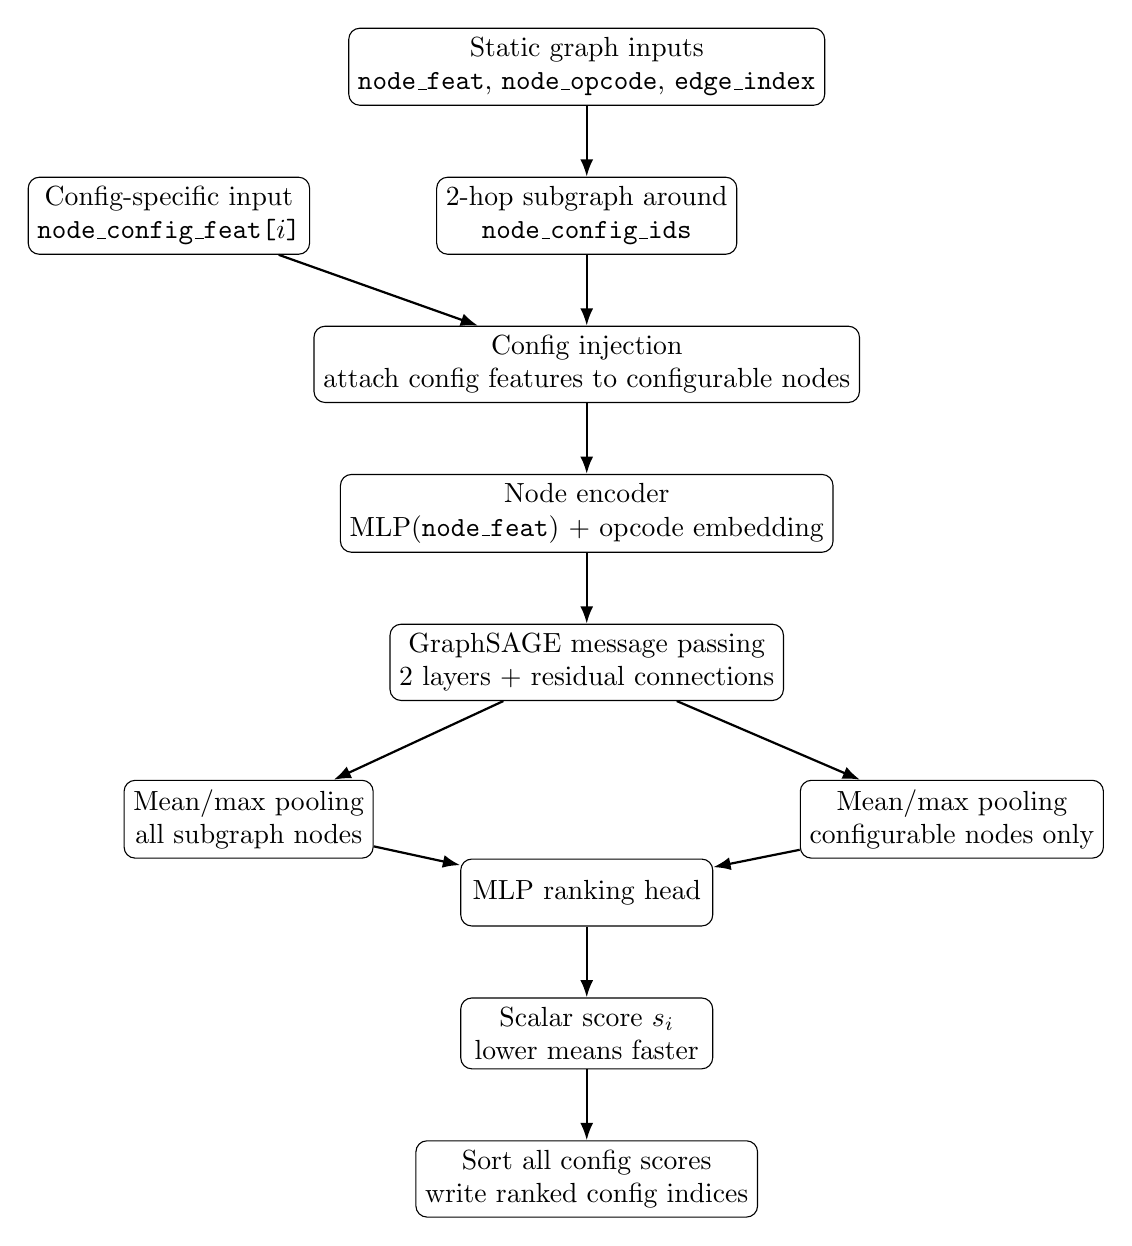
\begin{tikzpicture}[
    node distance=0.9cm and 1.15cm,
    box/.style={draw, rounded corners, align=center, minimum width=3.2cm, minimum height=0.85cm},
    smallbox/.style={draw, rounded corners, align=center, minimum width=2.7cm, minimum height=0.75cm},
    arrow/.style={-{Latex[length=2.2mm]}, thick}
]

\node[box] (graph) {Static graph inputs\\\texttt{node\_feat}, \texttt{node\_opcode}, \texttt{edge\_index}};
\node[box, below=of graph] (subgraph) {2-hop subgraph around\\\texttt{node\_config\_ids}};
\node[box, left=1.6cm of subgraph] (config) {Config-specific input\\\texttt{node\_config\_feat[$i$]}};
\node[box, below=of subgraph] (inject) {Config injection\\attach config features to configurable nodes};
\node[box, below=of inject] (encoder) {Node encoder\\MLP(\texttt{node\_feat}) + opcode embedding};
\node[box, below=of encoder] (sage) {GraphSAGE message passing\\2 layers + residual connections};
\node[smallbox, below left=1.0cm and 0.2cm of sage] (globalpool) {Mean/max pooling\\all subgraph nodes};
\node[smallbox, below right=1.0cm and 0.2cm of sage] (configpool) {Mean/max pooling\\configurable nodes only};
\node[box, below=2.0cm of sage] (head) {MLP ranking head};
\node[box, below=of head] (score) {Scalar score \(s_i\)\\lower means faster};
\node[box, below=of score] (rank) {Sort all config scores\\write ranked config indices};

\draw[arrow] (graph) -- (subgraph);
\draw[arrow] (config) -- (inject);
\draw[arrow] (subgraph) -- (inject);
\draw[arrow] (inject) -- (encoder);
\draw[arrow] (encoder) -- (sage);
\draw[arrow] (sage) -- (globalpool);
\draw[arrow] (sage) -- (configpool);
\draw[arrow] (globalpool) -- (head);
\draw[arrow] (configpool) -- (head);
\draw[arrow] (head) -- (score);
\draw[arrow] (score) -- (rank);

\end{tikzpicture}
\caption{Memory-safe graph-conditioned ranker for layout configurations.}
\end{figure}

\section{Why Each Component Exists}

\begin{table}[h]
\centering
\begin{tabular}{@{}p{0.28\linewidth}p{0.62\linewidth}@{}}
\toprule
\textbf{Component} & \textbf{Reason} \\
\midrule
Config injection &
The same graph has many configurations. Without injecting \texttt{node\_config\_feat},
all configurations for one graph would receive nearly identical scores. \\
\addlinespace
2-hop configurable-node subgraph &
Most layout-specific signal is near \texttt{node\_config\_ids}. A local subgraph
reduces RAM while keeping the nodes most directly affected by the compiler layout choice. \\
\addlinespace
GraphSAGE layers &
GraphSAGE can use edge-index message passing without constructing a dense
\(N \times N\) adjacency matrix. This is important for large graphs. \\
\addlinespace
Residual connections &
Residual updates make training more stable and reduce oversmoothing when multiple
message-passing layers are stacked. \\
\addlinespace
Configurable-node pooling &
Global pooling can dilute the layout signal. Pooling configurable nodes separately
keeps the representation focused on the nodes whose layout features changed. \\
\addlinespace
Scalar ranking head &
The competition needs an ordering of configurations, so the model only needs a
score that can be sorted. It does not need calibrated runtime predictions. \\
\bottomrule
\end{tabular}
\end{table}

\section{Ranking Objective}

For each graph, sample pairs of configurations \((c_f, c_s)\), where \(c_f\) is
faster than \(c_s\). The model should assign a lower score to the faster
configuration:
\[
s_f < s_s.
\]

A maximum-margin pairwise ranking loss is:
\[
\mathcal{L}
= \max(0, m + s_f - s_s),
\]
where \(m > 0\) is the margin. The loss is zero only when the faster
configuration is scored at least \(m\) lower than the slower configuration.

This objective is better aligned with the leaderboard than mean squared error,
because the submission is a ranking rather than an exact runtime estimate.

\section{RAM Strategy}

The first implementation should be designed around Colab memory limits:

\begin{itemize}
    \item Use a 1-hop or 2-hop induced subgraph around \texttt{node\_config\_ids}.
    \item Cap the subgraph size, for example \texttt{GNN\_MAX\_SUBGRAPH\_NODES = 512}.
    \item Never create a dense \(N \times N\) adjacency matrix.
    \item Use edge-index aggregation with \texttt{index\_add} style message passing.
    \item Start with small values such as \texttt{GNN\_BATCH\_SIZE = 4},
          \texttt{GNN\_HIDDEN\_DIM = 32}, and \texttt{GNN\_MAX\_EPOCHS = 3}.
    \item Sample a small number of configurations per file first, for example
          \texttt{32} to \texttt{64}, before scaling up.
\end{itemize}

\section{Initial Experiment Scope}

The first test should be limited to:
\[
\texttt{layout:xla:default}, \quad \texttt{layout:xla:random}.
\]

The GNN should be evaluated by the same validation ranking score as the existing
tree models. It should only be integrated into the final submission pipeline if
it improves validation on these layout collections.

\end{document}
